{\let\clearpage\relax\let\cleardoublepage\relax
\chapter{Disco protoplanetario}
}

Il materiale presente nella regione instabile di una nube molecolare \'e dotato di momento angolare quindi accresce s la massa della protostella centrale formando un disco ortogonale al momento totale della nube che trascurando l'effetto della pressione del gas, ruota con velocit\'a angolare kepleriana.

\begin{workout}[Refs dischi protoplanetari]
Chronology of  early stages: apai lauretta 10 (book)
\end{workout}

\section{Modello disco di accrescimento}

Nei modelli unidimensionali per disco di accrescimento si parametrizza viscosit\'a tramite $\nu=\frac{\eta}{\rho}\to\alpha c_s H$: giustifico euristicamente la parametrizzazione della viscosit\'a del disco di accrescimento in analogia alla viscosit\'a molecolare (\cite{bouvier2002theory}).

L'equazione del moto per un elemento di fluido
\begin{align}
&\PDof{t}(\rho v_i)+\PDof{x_i}(\rho v_iv_j+T_{ij})=F_i\\
&T_{ij}=P\delta_{ij}-\sigma_{ij}\\
&\sigma_{ij}=\eta(\partial_jv_i+\partial_iv_j-\frac{2}{3}\delta_{ij}\partial_kv_k+\zeta\delta_{ij}\partial_kv_k
\end{align}
dove $\eta$, $\zeta$ sono le shear and bulk viscosity, quest'ultima legata ai gradi di libert\'a interni della molecola \'e trascurabile se i tempi di equipartizione interni sono molto minori del tempo fra due collisioni.
%-$\sigma_{ij}$ \'e flusso di componente i di momento in direzione j
Considero la velocit\'a istantanea di una molecola nel piano xy $(v_x+u_x,u_y)$, dove u \'e la componente casuale e $\exv{}$ rappresenta valore mediato su grande numero di particelle/tempo (agitazione termica: $\exv{u}=0$) quindi
\begin{equation}
\sigma_{xy}=-\rho\exv{u_xu_y}
\end{equation}
dove ho preso la media temporale.
D'altra parte la forza viscosa agente sulla molecola \'e
\begin{equation}
F_{visc,x}=\TDy{y}{\sigma_{xy}}\approx\TDof{y}(\eta\TDy{y}{v_x})
\end{equation}
con $\eta=\rho\nu$.
%PRIM'ORDINE IN \lambda/L
Dalle equazioni precedenti si ha che
\begin{equation}
\exv{u_iu_j}=-\nu\TDy{x_j}{v_i}
\end{equation}

Per un disco di densit\'a superficiale $\Sigma(r,t)$, dotato del campo di velocit\'a $(u_r,r\Omega+u_{\phi})$, scrivo le equazioni di conservazione di massa e la componente azimutale dell'equazione del moto
\begin{align}
&\PDy{t}{\Sigma}+\frac{1}{r}\PDof{r}(r\Sigma v_r)=0\\
\Sigma(\PDy{t}{v_{\phi}}+v_r\PDy{r}{v_{\phi}}\frac{v_rv_{\phi}}{r})=0
\end{align}
da cui segue l'equazione del momento angolare
\begin{equation}
\PDof{t}[r\Sigma(r\Omega+u_{\phi})]+\frac{1}{r}\PDof{r}[r^2\Sigma(r\Omega+u_{\phi})u_r]=0
\end{equation}
infine, mediando le fluttuazioni su scala spaziale opportuna e trascurando la fluttuazione azimutale nel termine di derivata temporale, ottengo l'equazione
\begin{equation}
\PDof{t}r^2\Sigma\Omega+\frac{1}{r}\PDof{r}[r^3\Sigma\Omega\exv{u_r}+\Sigma r^2\exv{u_ru_{\phi}}]=0
\end{equation}
che rappresenta un fluido viscoso di velocit\'a $\vec{v}=(u_r,\Omega r)$ tensore degli stress $\sigma_{r\phi}=-\Sigma\exv{u_ru_{\phi}}$.

Per semplicit\'a si parametrizza il trasporto di momento angolare ponendo $\nu=\alpha c_s H$ dove $\alpha$ \'e parametro da fissare, $c_s$ la velocit\'a del suono e H lo spessore del disco:
\begin{equation}
\PDy{t}{\Sigma}=3\frac{1}{r}\PDof{r}[r\expy{1/2}\PDof{r}(\nu\Sigma r\expy{1/2})]\label{eq:sigmaevol}
\end{equation}

Nella popolazione planetaria simulata $\alpha$ \'e fissato sulla base delle osservazioni  ed \'e omogeneo e costante.

\begin{workout}[Viscous/turbulent disk]
laminar (high momentum diffusion)
mass inflow Gullbring98 \SIrange{e-9}{e-7}{\per\year}$\msun{}$
\end{workout}


\begin{workout}[MRI]
fig 10.3:
gammie 1996
\end{workout}


\begin{workout}[Accretion disk sources]
o218, 296: disk formation, constrains from solar system
the alpha disk pg 18: theory of turbulent accretion disk
\end{workout}

\begin{workout}[Isothermal cloud collapse!]

\end{workout}


\begin{workout}[Intro a disco accrescimento]
Nei modelli globali la formazione planetaria \'e simulata partendo dalla fase finale di accrescimento di massa sulla stella centrale (per semplicit\'a considero stelle di $1\msun{}$ singole): il collasso di nube molecolare produce strutture appiattite la cui evoluzione \'e determinata dal trasporto di momento angolare verso l'esterno, l'interazione con l'oggetto centrale (campi magnetici vento stellare) e con l'ambiente circostante.
L'ipotesi su cui si basano le simulazioni considerata \'e che la componente polverosa formi corpi pi\u massicci fino a masse di frazioni di masse terrestri  ed infine accrescere gas: lo scenario di core accretion (CA).
\end{workout}

\begin{workout}[Modelli 1D disco accrescimento: struttura verticale]
auto gravitazione trascurabile quindi la struttura verticale \'e determinata dalla componente lungo z dell'attrazione del corpo centrale, profilo termico determinato da equilibrio.
\end{workout}

\begin{workout}[Descrizione trasporto momento angolare tramite parametrizzazione viscosit\'a]
Mass conservation + momentum conservation in viscous flow: angular momentum evolution. Phenomena: Shear viscosity - turbulence - MRI.
Nei modelli 1D per disco di accrescimento si parametrizza viscosit\'a tramite $\nu=\frac{\eta}{\rho}\to\alpha c_s H$: la viscosit\'a molecolare \'e troppo bassa  per trasportare all'esterno il momento angolare sui tempi-scala osservati.

Theory of turbulent accretion disk: pg 18, 8.
Flusso di x-momentum lungo y $\rho\exv{u_xu_y}$, dove considero la velocit\'a dell'elemento di fluido $(v_x+u_x,u_y)$ dove le $u$ rappresentano fluttuazioni della velocit\'a: $\sigma_{xy}=-\rho\exv{u_xu_y}$.
Ricordando la definizione di tensore degli stress e con $\vec{v}=v_x(y)\hat{x}$

\begin{equation}
\sigma_{ij}=\eta(\partial_jv_i+\partial_iv_j-\frac{2}{3}\delta_{ij}\partial_kv_k+\zeta\delta_{ij}\partial_kv_k \to \eta\TDy{y}{v_x}
\end{equation}

\begin{equation}
\PDof{t}(\rho v_i)+\PDof{x_i}(\rho v_iv_j+T_{ij})=F_i
\end{equation}
Fluttuazioni: $\sigma_{ij}=-\rho\exv{u_iu_j}$.
Viscosit\'a molecolare: $\exv{u_iu_j}=-\nu\TDy{x_j}{v_i}$.
Turbulence: Reynpold stress $\tau_{ij}=-\rho\exv{v_jv_i}$, $\exv{u_iu_j}=-\nu_T\TDy{x_j}{v_i}$
\begin{equation}
\PDy{t}{\Sigma}=3\frac{1}{r}\PDof{r}[r\expy{1/2}\PDof{r}(\nu\Sigma r\expy{1/2})]\label{eq:sigmaevol}
\end{equation}
\end{workout}

\begin{workout}[Photoievaporation: X-EUV-FUV (Alexander13: The Dispersal of Protoplanetary Disks)]
Protoplanetary disc evolution and dispersal: the implications of X-ray photoevaporation
\end{workout}

\begin{workout}[alpha prescription]
$\vec{v}=(u_r,r\Omega)$, stress tensor $\sigma_{r\phi}=-\Sigma\exv{u_ru_{\phi}}$.
Enhanced turbulent viscosity: $-\Sigma\exv{u_ru_{\phi}}=\Sigma\nu r\TDy{r}{\Omega}$, $\nu=v_TH$, $\alpha=v_T/c_s$
\end{workout}

\begin{workout}[Modello di disco di accrescimento - (Mordasini18: 4) - Introduzione descrizione fenomeni grazie a PPS]
Un modello di disco  di accrescimento usato nelle simulazioni considera l'evoluzione della densit\'a superficiale tramite l'equazione \eqref{eq:diskaccrphev-m18}

\begin{align}
&\TDy{t}{\Sigma}=\frac{1}{r}\PDof{r}[3r\expy{1/2}\PDof{r}(\nu\Sigma r\expy{1/2})]+\dot{\Sigma}_w(r)+\dot{\Sigma}_p(r)\label{eq:diskaccrphev-m18}\\
&\dot{\Sigma}_w(a)=\left\{\begin{array}{c}0\\\frac{\dot{M}_w}{2\pi(a_{max}-R_g)a}\\\end{array}\right.
\end{align}

Densit\'a superficiale iniziale:
\begin{equation}
\Sigma(a,t=0)=\Sigma_0(\frac{r}{1AU})\expy{p_g}\Exp{[-(\frac{r}{R_o})\expy{2+p_g}]}(1-\sqrt{\frac{r}{R_i}})
\end{equation}
4-Mordasini18 (Hayashi81). $p_g\approx1$ (Andrews10).
\end{workout}


\begin{workout}[Foto-evaporazione]
(Photoevaporation: veras armitage 2003, Alexander13, Mordasini12. Internal/External).
EUV($E\approx13.6eV$): ionization, FUV($E\approx6-13.6eV$): dissociation, X-ray
\end{workout}

\section{YSO: distribuzione propriet\'a dischi protoplanetari}

\begin{workout}[YSO: classificazione ]
SED: emissine a lunghezze d'onda millimetriche probano tutto il volume del disco, otticamente sottile a quelle lunghezze (Beckwith 90, Beckwith Sargent91).
$S_{\nu}\propto B_{\nu}(1-\exp{-\tau})\approx B_{\nu}\tau$: emission produced near cold disk mid-plane.
Rayleigh-jeans: $B_{\nu}\propto T$ and, since $\tau=\kappa\Sigma$, $S_{\nu}\propto \kappa\Sigma T$.
(SED: Andrews williams 07)
Survey: 0.3'', 345Ghz(870$\micro m$) 1Myr old Ophiuchus stars forming region
Se la viscosit\'a \'e statica e distribuita secondo $\nu\propto r\expy{\gamma}$:
\begin{align}
&R_c=R_1\mathcal{T}\expy{1/(2-\gamma)}\\
&M_d=M_{d,0}\mathcal{T}\expy{-1/2(2-\gamma)}\\
\end{align}
\end{workout}

\begin{workout}[YSO properties distro]
Refs: ''Protoplanetary Disk Structures in Ophiuchus''
da dove sono ricavete nei PPS?
mass: MMSN, andrews 10, manara 16
lifetime: IR/UV excess: haisch 01, mamajek 09
initial embryo starting position: relative spacing of few hill radii (kokubo ida 00), fill disk thinking of asyntituc isolation mass (Ida Lin 10), trapped (hasegawa pudritz 11, cridland 16)
Hueso 05: evolution of protoplanetary disk, meyer 06 Formation and evolution of planetary systems, Udry 07: statistical properties of exoplanets)
Distribuzione di probabilit\'a per condizioni iniziali.
Initial condition for planet formation (protoplanetry disk \cite{meyer2006formation}): disk metallicity, mass, lifetime, \ldots

{Metallicity and Dust/Gas}
$[M/H]$ distro modelled as normal: $\mu=-0.02$, $\sigma=0.22$ (photosphere of solar-like stars in solar neighborhood): Santos05.
$f_{dg}=f_{dg,\odot}10\expy{[M/H]}$ with $f_{dg,\odot}=0.01-0.02$.

Initial disk mass
(infall phase end, no more self-gravitational instabilities) - stability(shu90), MMSN hayashi81/weidenshilling77, observations(Andrews10,Manara16) points to $(0.1-10)\%$ stellar mass, distro log-normal with mean $0.01M_*$.

{Disk lifetime}
$1-10My$ with mean $3My$ (Haisch01, Mamajek09)

{Embryo starting position}
Usually a distro uniform in log(a): relative spacing of few Hill spheres (Kokubo Ida 10)
Ida, lin10: asymptotical isolation mass ''Toward a Deterministic Model of Planetary Formation VI'',
Trapped evolution model: Hasegawa pudritz 11, Cridland 16

\end{workout}

\begin{workout}[Refs dischi protoplanetari]
Ciesla Dullemond10 
Perryman ch 10
williams cieza 11
Andrews 09-10
mamajek 2009 - Initial conditions of planet formation: lifetimes of primordial disks
infrared excess: gail hoppe10
\end{workout}

\begin{workout}[Classificazione YSO: convenzioni]
Sorgenti con SED declinante in mid infrared ($2.5-10\si{\micro\meter}$): $1.5<\alpha_{IR}=<0$. Active/passive: mass infall convert G into thermalradiation/reprocessed starlight.
Refs: Perrymann 10.3 - disk formation pg 218 - 
Classification based on slope of SED between $2-25\si{\micro\meter}$: $\alpha_{IR}=\TDly{\nu}{\nu F_{\nu}}=$ (Gail Hoppo 2010)
Spitzer: forming regions within 500pc
Formation: disk quickly forms as more distant material with high angular momentum, centrifugal radius $R(t)\propto\Omega^2 t^3$: . Class 0-I : protostellar disk, gravitational unstable (cloud collapse: the collapse of the cores of slowly rotating isothermal clouds, Terebey shu cassen 1984, selfsimilar collapse of isothermal spheres and star formation, shu 77). Singular isothermal sphere: $\rho=\frac{a^2}{2\pi G}r\expy{-2}$, $M(r)=\frac{2a^2}{G}r$
\end{workout}


{\let\clearpage\relax\let\cleardoublepage\relax
\chapter{Schema di formazione planetaria per core accretion}
}

\begin{workout}[Refs GI vs CA]
planetesimal hypoithesis: chamberlin 05, Safronov 69, Hayashi 77. Formation on dynamical scale via GI: Kuiper 51, Cameron 62.
Core accretion o instabilit\'a gravitazionale?
La correlazione tra metallicit\'a del disco protoplanetario e il numero di pianeti (giganti) \'e in accordocon osservazioni?
\end{workout}


Il modello di formazione planetaria da me considerato, si basa sulla sedimentazione della componente polverosa nel disco protoplanetario in embrioni planetari che, se abbastanza massicci sono in grado di accrescere il gas presente nel disco protoplanetario.

L'altro schema di formazione considera l'instabilit\'a gravitazionale del disco. 

Esistono alcuni dati osservativi in favore del primo modello, considerando il sistema solare: arricchimento dei pianeti del sistema solare rispetto a composizione solare di metalli (la composizione di Urano/Nettuno contiene $1\%$ di $H_2$, $He$ contenuto in pianeta di composizione solare con pari massa di metalli), ipotizzando una rimozione della parte gassosa il pianeta deve avere il tempo di sedimentare la componente metllica, \'e necessario un disco di massa solare e i pianeti si formerebbero a distanza maggiore, non spiega la formazione dei corpi minori.

\section{Sedimentazione polvere e formazione planetesimi}

Si ha la condensazione della polvere in corpi dominati da autogravitazione, in \SIrange{e4}{e5}{\year}.

L'equazione del moto per particella di polvere \'e
\begin{equation}
m_p\TDy{t}{v_z}=F_D-m_p\Omega^2z
\end{equation}
$F_D$ \'e la forza esercitata dal gas sulla particella di polvere
\begin{equation}
F_D=-\frac{1}{2}C_D\pi s^2\rho_gv^2
\end{equation}
nel caso cammino libero medio delle molecole di gas sia maggiore delle dimensioni della particella $C_D=\frac{8}{3}\frac{v_{th}}{v}$ (Epstein drag).
Grani piccoli raggiungono rapidamente la velocit\'a stazionaria di regime
\begin{equation}
v_{set}=\frac{\Omega^2}{v_{th}}\frac{\rho_d}{\rho_g(z)}sz
\end{equation}
La formula precedente prevede sedimentazione per particella mm in 100: risultano evidenze contrarie dalle osservezioni.

Inoltre l'eventuale scambio di momento tra gas e polvere dovuto alla velocit\'a di rotazione minore di quella kepleriana del gas:
\begin{equation}
g_{eff}=-\frac{GM_*}{r^2}-(\frac{1}{\rho_g}\TDy{r}{P}=r\Omega_g^2
\end{equation}
$\Omega_g$ \'e $\approx0.5\%$ di quella kepleriana.

Per passare a corpi di dimensioni kilometriche si ipotizzano 2 scenarii:
\begin{itemize}
\item La componente solida del disco di accrescimento sedimenta rapidamente in disco sottile: secondo il modello di Goldreich-Ward il disco di polvere \'e instabile e le condensazioni generano i planetesimi.
\item In assenza di sedimentazione la formazione procede tramite urti a 2 corpi e la turbolenza creando addensamenti, pu\'o accelerare la formazione di planetesimi.
\end{itemize}

\begin{workout}[Dust settling model]
Furlan 06: Effects of dust growth and settling in T Tauri disks
Nomura 06: Dust Size Growth and Settling in a Protoplanetary Disk
\cite{lissauer1993planet}
 \end{workout}

\begin{workout}[Dust dynamics refs]
Weidenschilling cuzzi 06: Particle-gas dynamics and primary accretion, Apai Lauretta Protoplanetary Dust pg 100
Protoplanetary disk and their evolution pg 29
Protoplanetary dust: Apai Lauretta - particles dynamics pg 100
\end{workout}

\begin{workout}[Particle-gas dynamics. dust midplane sedimantation]
Weidenschilling cuzzi 06: Particle-gas dynamics and primary accretion, Apai Lauretta Protoplanetary Dust pg 100
Stopping time $t_s=\frac{\rho_sa}{\rho c_s}$ ($a<\lambda_g$). L'evoluzione dinamica delle particelle solide \'e determinata flussi macroscopici dovuti all'evoluzione del disco, gas-drag, settling
\end{workout}

\begin{workout}[Formazione planetesimi: meccanismo Goldreich-Ward]
Weidenschilling cuzzi 06: Particle-gas dynamics and primary accretion, Apai Lauretta Protoplanetary Dust pg 100
Stopping time $t_s=\frac{\rho_sa}{\rho c_s}$ ($a<\lambda_g$). L'evoluzione dinamica delle particelle solide \'e determinata flussi macroscopici dovuti all'evoluzione del disco, gas-drag, settling
\end{workout}

\section{Accrescimento planetsemi: formazione proto-pianeti.}


\begin{figure}[!t]
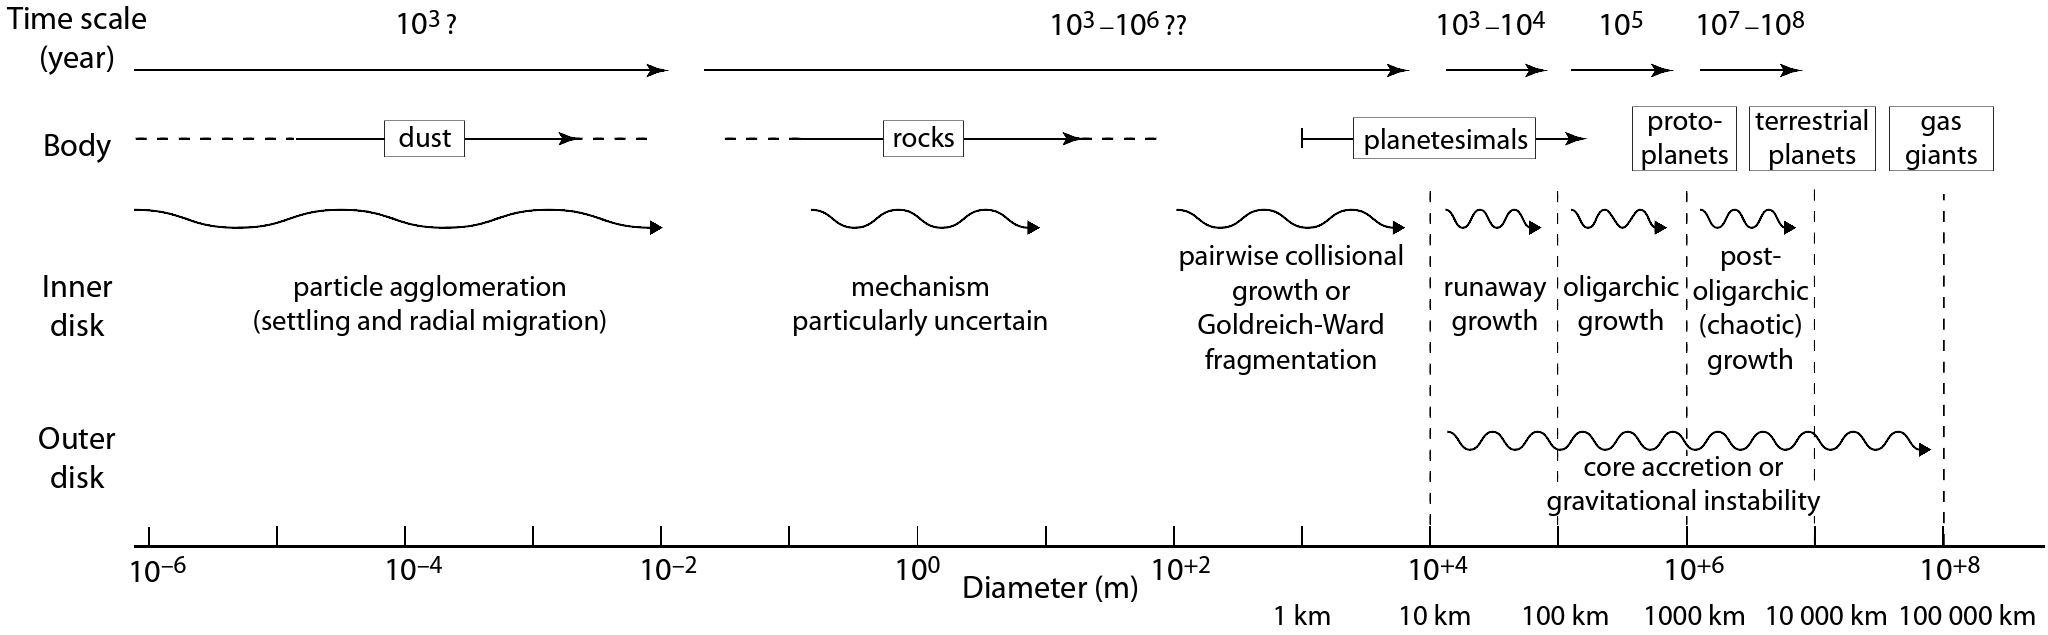
\includegraphics[width=0.9\textwidth]{accretiontimeline}
\end{figure}

\begin{workout}[Dynamical evolution of planetesimal swarm: refs]
Accretional evolution of planetesimal swarm (weidenschilling 97)
\end{workout}

\begin{workout}[10m-10km, 100km-1000km, 1000km-10000km: refs]
Lissauer pg 142-143
Perryman pg 226
\end{workout}

\subsection{Distribuzione planetesimi}

La popolazione dei planetesimi evolve attraverso interazione con gas e scattering/collisioni con planetesimi: l'interazione tra planetesimi trasforma il moto kepleriano in casuale e si ha equipartizione di energia tra pianetesimi di diversa massa; i planetesimi di massa minore hanno maggiore dispersione di velocit\'a, l'interazione col gas smorza eccentricit\'a e inclinazione inoltre due planetesimi hanno stessa velocit\'a relativa primo e dopo interazione ma aumenta la velocit\'a relativa al moto kepleriano in maniera casuale.

\'E ragionevole supporre che si arrivi rapidamente alla condizione $v>\Omega R_H$.

\begin{workout}[Planetesimal dynamics: viscous stirring]
The origin of anisotropic velocity dispersion of particles in a disc potential (Ida, Makino 93, Stewart-Wetherill 1988 Ida1990)
\end{workout}

\begin{workout}[Gravitational stirring: Viscous stirring and dynamical friction]
\begin{itemize}
\item Viscous stirring increses i,e
\item Dynamical stirring: tends to equalize energy of random motion among bodies having different masses and velocities
\end{itemize}
\end{workout}

\begin{workout}[orbital elements distribution: raylegh distro]
\begin{equation}
I planetesimi hanno distribuzione di velocit\'a casuale, localmente equivalente a
f(e,i)=4\frac{\sigma}{m}\frac{ei}{\exv{e^2}\exv{i^2}}\Exp{[-\frac{e^2}{\exv{e^2}}-\frac{}{\exv{i^2}}]}
\end{equation}
\'e una distro gaussiana triassiale in coordinate cilindriche (Lissauer Stewart 93)
Lissauer pg 142-143
\end{workout}

\subsection{Regimi accrescimento dei protopianeti}

L'accrescimento di massa del protopianeta procede secondo
\begin{equation}
\TDy{t}{M_e}=\pi R_c\Sigma_p\Omega F_g
\end{equation}
$F_g$ \'e determinato dalla velocit\'a relativa tra proto-pianeta e planetesimi.

\begin{workout}[Protoplanets accretion of solids]
Other refs: Planet formation coagulation: focus on U,N (Goldreich 04), Final stages of planets formation (Goldreich 04), Formation of giant planets core: evaluating key processes (levison 09).
Safronov69: $\dot{M}_c=\Omega\Sigma_pR^2_{capture}F_G$, $R_{capture}$ larger than core radius due to gas drag, $F_G(e,i)$ gravitational focus (give rise to different growth regimes: runaway, oligarchic, orderly).
Runaway growth until protoplanets $100-1000km$ (dep on position).
Oligarchic growth: velocity of planetesimal raised by viscous stirring (gravitational scattering)/ damped by gas (until disk present).
Enhanced radius by atmospheric drag: Enhanced collisional growth of a protoplanet that has an atmosphere (Inaba Ikoma 03)
\end{workout}

\begin{workout}[orderly growth]
lissauer pg 144: equapartition effect saturation. This regime is never observed in simulations.
\begin{equation}
\frac{1}{m_p}\TDy{t}{m_p}\propto m_p\expy{-1/3}
\end{equation}
\end{workout}

\begin{workout}[runaway growth]
\begin{equation}
\frac{1}{m_p}\TDy{t}{m_p}\propto m_p\expy{1/3}
\end{equation}
\end{workout}

\begin{workout}[feeding zone]
Jacobi integral:
\begin{align}
&E_J=\frac{1}{2}(e^2+i^2)a^2\Omega^2-\frac{3}{8}b^2\Omega^2+\frac{9}{2}R_H^2\Omega^2\\
&\tilde{E}_J=\frac{E_J}{a^2h^2\Omega^2},\ h=R_H/a
\end{align}
Planetesimi con $\tilde{E}_J>0$ possono accrescere il protopianeta  cio\'e entro $w_{feed}=B_LR_H$, per orbite circolari $B_L=2\sqrt{3 }$.
\end{workout}

\begin{workout}[runaway to oligarchic. Isolation mass]
 NEW CONDITION FOR THE TRANSITION FROM RUNAWAY TO OLIGARCHIC GROWTH (Ormel 10)
 \begin{equation}
M_{iso}\propto M_*\expy{-1/2}\Sigma_p\expy{3/2}r^3
\end{equation}
$0.07\mearth{}$ 1AU, $9\mearth{}$ 5 AU.
\end{workout}
  
\begin{workout}[Accrescimento pianetesimi: orderly, runaway, oligarchic]
The growth of planetary embryos:  orderly, runaway, or oligarchic? (Rafikov 2002)
\begin{align}
\TDy{t}{M_e}\approx\pi R_e^2\Omega mN\frac{v}{v_z}[1+\frac{2GM_e}{R_ev^2}]
\end{align}
Accrescimento ordinato: $\frac{1}{M_e}\TDy{t}{M_e}\propto M_e\expy{-1/3}$. Accrescimento runaway: $\frac{1}{M_e}\TDy{t}{M_e}\propto M_e\expy{1/3}$. Accrescimento oligarchico: $\frac{1}{M_e}\TDy{t}{M_e}\propto M_e\expy{-1/3}$.
\end{workout}

\begin{workout}[Timescale of oligarchic growth]
kokubo ida 02 (ida lin 04)
\begin{align}
&\dot{M}_c=\frac{M_c}{\tau_c}\\
&\tau_c=\SI{1.2e5}{\year}(\frac{\Sigma_p}{\SI{10}{\gram\per\cubic\cm}})\expy{-1}(\frac{a_p}{\SI{1}{\astronomicalunit}})\expy{1/2}(\frac{M_p}{\mearth{}})\expy{1/3}(\frac{M_*}{\msun{}})\expy{-1/6}[(\frac{\Sigma_g}{\SI{2400}{\gram\per\cubic\cm}})\expy{-1/5}(\frac{a_p}{\SI{1}{\astronomicalunit}})\expy{1/20}(\frac{m}{\SI{e18}{\gram}})\expy{1/15}]^2
\end{align}
\end{workout}

\begin{workout}[Post-oligarchic growth: 1000km-10000km]
Chaotic growth until stable configuration is reached.
Factors determning orbital spacing: pg 229, earth formation (chambers 01, raymond 05, o'brian 06)
\end{workout}

\chapter{Accrescimento gas}

Refs: Planet formation models: the interplay with the planetesimal disc (Fortier 2013), Characterization of exoplanets from their formation I. Models of combined planet formation and evolution (Mordasini 12)

Si risolvono numericamente le equazioni di conservazione di massa, equilibrio idrostatico, conservazione/trasporto energia 1D

\begin{workout}[Attached phase: boundary conditions]
\begin{align}
&P_{pl}=P_{Neb}\\
&T_{Pl}=T_{Neb}\\
&R_{Pl}=Min(R_H,R_H)
\end{align}
\end{workout}


\begin{workout}[Detached phase: transition condition and boundary condition]
Transition attached/detched phase $\approx10\mearth{}$.
Accretion shock for free-falling materials from Hill radius (more realistic circumplanetary disk: Papailoizou Nelson 05)
\begin{align}
&\dot{M}_{XY}^{max}\\
&v_{ff}^2=2GM(\frac{1}{R}-\frac{1}{R_H})\\
&P=P_{neb}+\frac{\dot{M}_{XY}}{4\pi R^2}v_{ff}+\frac{2g}{3\kappa}\\
&\tau=max(\rho_{neb}\kappa_{neb}R,2/3)\\
&T^4_{int}=\frac{3\tau L_{int}}{8\pi\sigma R^2},\ T^4=(1-A)T_{neb}^4+T_{int}^4
\end{align}
$R\approx1.5-5\rjupiter{}$ depending on entropy: THE PLANETARY ACCRETION SHOCK:I. FRAMEWORK FOR RADIATION-HYDRODYNAMICAL SIMULATIONS AND FIRST RESULTS (m17), Characterization of exoplanets from their formation III: The statistics of planetary luminosities (m17)
Bondi accretion rate: $\dot{M}_{e, Bondi}\approx\frac{\Sigma}{H}(R_H/3)^3\Omega$ or viscous accretion rate $\dot{M}_{e, visc}\approx f_{lub}3\pi\nu\Sigma_g$
\end{workout}

\begin{workout}[Higher mass gap formation reduces accretion rate]
\begin{equation}
f_{va04}=1.668(\frac{M_p}{\mjupiter{}})\expy{1/3}\exp{-\frac{M_p}{1.5\mjupiter{}}}+0.04
\end{equation}
\end{workout}

\begin{workout}[Planet-Disk exchange in hydrodynamic manner]
Ormel 15/ Cimerman 17
\end{workout}


\chapter{Migrazione}

\begin{workout}[Migration refs]
Refs: \cite{ward1997protoplanet}, \cite{terquem2000disks}, \cite{menou2004low}, (
Planet-disk interaction and orbital evolution (kley Nelson 2012), 
Baruteau 2016)
crida06: On width and shape of gaps in PPD,crida phd, 
Trilling 98:Orbital evolution and migration of giant planet: modellingextrasolar planets (Angular momentum injection rate, torque from spinning star, Impact of planet migration models on planetary populations)
Dittkrist 14: Impact of planetsmigration models n planetarypopulation (Migration II inward/outward: non equilibrium gas flow, problem of isothermal disk migration timescale: migration I regime, Fig 7,
\end{workout}

Il disco di accrescimento esercita momento torcente sul pianeta che produce un trasferimento di momento angolare dal pianeta al disco $\Lambda(a,R)$
\begin{align*}
&J=M_p\sqrt{GM_*a_p}\\
&\TDy{t}{a}=2a_p\frac{\Gamma_t}{J}=-(\frac{a}{GM_*})(\frac{4\pi}{M_P})\int_{r_{int}}^{r_{out}}r\Lambda\Sigma\,dr
\end{align*}
$r_{int}, r_{out}$ inner/outer disk radius (rif to disk ar planet)

\begin{workout}[Migration/resonance]
N-body, resonanceand migration
The dynamics of two massive planets on inclined orbits (Veras Armitage 04)
\end{workout}

\section{Migrazione tipo I: regime lineare}

Unperturbed disk: axisymmetric, keplerian rotation $\Omega(r)=\sqrt{GM_*/r^3}$, vanishing radial velocity. Planet potential, periodic in $\phi$, $\phi_p=\Omega_pt$:
\begin{align*}
&\psi_p(r,\phi,t)=-\frac{Gm_p}{|\vec{r}_p(t)-\vec{r}|}=\sum_{m=0}^{\infty}\psi_m(r)\cos{m[\phi-\phi_p(t)]}
\end{align*}
Total torque excertes by disk on planet
\begin{equation*}
\Gamma_t=-\int_{disk}\Sigma(\vecp{r}{F})\,df=\int_{disk}\Sigma(\vecp{r}\wedge\nabla\psi_p)\,df=\int_{disk}\Sigma\PDy{\phi}{\psi_p}\,df
\end{equation*}
$\Sigma$ surface density,  $\vec{F}$ specific force, $df$ surface element.
Whenever frequency of individual potential component as seen by fluid particle in disk $\omega=m(\Omega(r)-\Omega_p)$, matches a natural  oscillation frequency of the disk we have resonant condition: torques are calculated at resonant locations.


Lindblad (due to m-component of planet potential) and corotation torques:
\begin{align*}
&\Gamma_m^L=\left.\sign{(\Omega-\Omega_p)}\frac{\pi^2\Sigma}{3\Omega\Omega_p}(r\TDy{r}{\psi_m}+\frac{2m^2(\Omega-\Omega_p)}{\Omega}\psi_m)^2\right|_{r=r_L}\\
&\Gamma_m^C=\left.\frac{m\pi^2}{2}\frac{\psi_m}{r\TDy{r}{\Omega}}\TDof{r}(\frac{\Sigma}{B})\right|_{r=r_C}
\end{align*}

Differnetial Lindblad torque
$B=\frac{\kappa^2}{4\Omega}$ is the second Oort constant and represents z component of flow vorticity $\nabla\wedge\vec{v}|_z$

\begin{workout}[Migration I in isothermal disk: pressure. Adiabatic, irradiated?]
Low mass planet in isothermal disk: linear analysis of perturbed flow.
When pressure can't be neglected the resonance condition becomes $m(\Omega(r)-\Omega_p=\sqrt{\kappa^2(r)(1+\xi^2)}$ where $\xi=\frac{mc_s}{\Omega r}$ where we used isothermal sound speed and let $c_s=H\Omega$: for $m\to\infty$ L. res position becomes $r_L=r_p+\frac{2H}{3}$ (torque cutoff).

Linear. Occur if $R_H$ is smaller then H, disk scale heigth, and if viscous torque are dominant compared to gravitational torque.
Subtypes: locally isothermal, adiabatic, un/satured-corotation torque: cooling behaviour of gas (Baruteau masset08, Casoli masset 08, paardekooper10,kley 09); timescales: dittkrist 14.
Migration timescale in isothermal approx (ida lin 08 a:):
\begin{align*}
&\tau_I=\frac{1}{2.728+1.082p_{\Sigma}}(\frac{c_s}{a_p\Omega})^2\frac{M_*}{M_p}\frac{M_*}{a_p^2\Sigma_g}\Omega\expy{-1}\\
s&\dot{a}_p=-\frac{a_p}{\tau_I}
\end{align*}
Paardekooper10, Dittkrist14: total torque $\Gamma_t=\frac{1}{\gamma}(C_0+C_1p_{\Sigma}+C_2p_T)\Gamma_0$ where $C_i$ depends upon sub-regime.
Benitez Llambay 15: heating torque, Paardekooper14 Pierens 15: dynamic corotation torque.
\end{workout}

\section{Massive enough planet to open gap: migration II}

Refs: On the tidal interaction between protoplanets and the primordial solar nebula. II - Self-consistent nonlinear interaction (1986)
Non-linear. For larger planet mass, when disk density distro is changed cons., the linear hteory is no more adeguate. If angular momentum isdeposited locally (viscous dissipation/shock waves)  the disk receeds from planets
Ida-lin04: angular momentum trasport in viscous accretion disk without planets that in type II migration act as relays that transmit angular momentum at that rateacross their gap via tidal torques.
Alibert05: the planet follow the gas except when massive than local disk.
Duffell14, Durmann kley 15: questioning that migration II follows viscous evolution of the disk but due to torque??


Planet-disk interactions: exchange of angular momentum. Low mass planet-linear theory.(''Planet-disk interactions and orbital evolution'')
Low mass planets: Lindblad and corotation torque. Rapid migration of intermediate mass planets. Gap forming massive planets: slower migration determined by viscous evolution of disk. (Role of disk self-gravity and MHD turbulence as function of planet mass).


\section{Migrazione III:}
Planet-disk interactions: exchange of angular momentum. Type III migration: planet of intermediate mass. (‘’Planet-disk interactions and orbital evolution’’).

Flow-through corotation torque: $\Gamma_{flow}=2\pi\Sigma_s\dot{a}_p\Omega_pa_p^3x_s$.

\begin{align*}
&\dot{a}_p=\frac{2\Gamma^L}{\Omega_pa_p(m_p’-\delta m)}
\end{align*}

\section{Eccentricity and inclination evolution}
Planet-disk interactions: normal, tangential, radial forces. eccentricity and inclination evolution. (‘’Planet-disk interactions and orbital evolution’’)
Decomposition of planet’s potential: non-circular orbit
\begin{align*}
&\psi_p(r,\phi,t)=-\frac{Gm_p}{|\vec{r}_p(t)-\vec{r}|}=\sum_{m=0}^{\infty}\sum_{n=-m}^m\psi_{m,n}(r)\cos{m\phi+(n-m)\Omega_pt]}
\end{align*}

Eccentricity damping.
For each m,n there are 3 resonant locations: external L resonance act to increase, corotation res. to damp (if unsaturted), and coorbital L res damp $e_p$. Linear analysis for low mass planets indicates rapid exponential damping of $e_p$:
\begin{align*}
&\TDy{t}{e_p}\propto-e_p,\ \tau_e\approx(\frac{H}{r})^2\tau_{mig}\\
&e_P>\frac{H}{r}: \TDy{t}{e_p}\propto-e_p\expy{-2}
\end{align*}
Risultati analoghi per inclinazione.
